%Plan et documentation de déploiement

%déploiement sur appbase.io

\subsection {Moteur de recherche}



%Le moteur de recherche fonctionne comme machin machin machin
Afin d'importer nos données, nous devons respecter le format JSON.
Dans un premier temps, nous créons une application depuis Appbase.io. 
Un Json se compose de plusieurs documents où chaque document est enlacé par des accolades.
Dans un document, nous avons des "fields" (champs) qui correspondent aux différentes familles de données récoltés.
Dans notre cas, nous avons comme exemple de champs les noms, les arrêtés ou les numéros de recueils. La structure du JSON est la suivante :


\begin{figure}[h!]
  \centering
	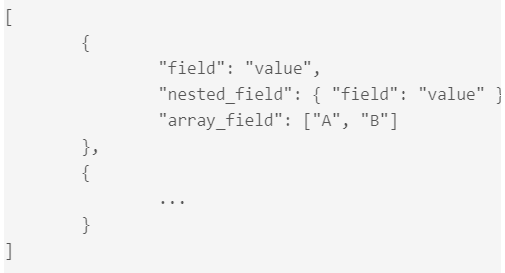
\includegraphics[width=0.5\textwidth]{FormatJsonAppbase.PNG}
	\caption[]{Exemple de format accepté sous Appbase}
  \label{}
\end{figure}

Lorsque les données sont correctement importé un mail est envoyé contenant le "credentials" (identifiant) afin de sécuriser l'accessibilité aux données. 
Les données sont visibles sous la forme d'un tableau. Cela nous permet de visualiser ce qui a été importé. 
Depuis l'onglet « search preview » nous avons une première visualisation du moteur de recherche. Depuis la bar de recherche généré, nous pouvons spécifier les champs qui sont recherchables.

